\chapter{Implementation\label{cha:chapter5}}

This chapter details the testbed implementation. It provides insight into the code of the Producer, Signer, Distributor and Consumer components, as well as the challenges I came across.

\section{Environment\label{sec:env}}

The following hardware and software has been used during the development process:

\begin{table}[H]
    \centering
    \begin{tabular}{l|lll|}
        \cline{2-4}
                                                                                                   & \multicolumn{1}{l|}{\textbf{Work Laptop 1}}                                               & \multicolumn{1}{l|}{\textbf{Work Laptop 2}}                                              & \textbf{Private Laptop}                                        \\ \hline
        \multicolumn{1}{|l|}{\textbf{Vendor}}                                                      & \multicolumn{1}{l|}{\begin{tabular}[c]{@{}l@{}}Lenovo ThinkPad \\ L14 Gen 4\end{tabular}} & \multicolumn{1}{l|}{\begin{tabular}[c]{@{}l@{}}Lenovo ThinkPad \\ P1 Gen 7\end{tabular}} & \begin{tabular}[c]{@{}l@{}}Framework \\ Laptop 13\end{tabular} \\ \hline
        \multicolumn{1}{|l|}{\textbf{\begin{tabular}[c]{@{}l@{}}Operating \\ System\end{tabular}}} & \multicolumn{1}{l|}{Ubuntu 24.04.1 LTS}                                                   & \multicolumn{1}{l|}{Ubuntu 24.04 LTS}                                                    & Ubuntu 24.04.2 LTS                                             \\ \hline
        \multicolumn{1}{|l|}{\textbf{CPU}}                                                         & \multicolumn{1}{l|}{Intel i7 1355U}                                                       & \multicolumn{1}{l|}{\begin{tabular}[c]{@{}l@{}}Intel Core Ultra \\ 9 185H\end{tabular}}  & Intel i5 1340p                                                 \\ \hline
        \multicolumn{1}{|l|}{\textbf{GPU}}                                                         & \multicolumn{1}{l|}{integrated}                                                           & \multicolumn{1}{l|}{\begin{tabular}[c]{@{}l@{}}NVIDIA RTX 4070\\ Mobile\end{tabular}}    & integrated                                                     \\ \hline
        \multicolumn{1}{|l|}{\textbf{RAM}}                                                         & \multicolumn{1}{l|}{32 GB}                                                                & \multicolumn{1}{l|}{64 GB}                                                               & 32 GB                                                          \\ \hline
        \multicolumn{1}{|l|}{\textbf{Browser}}                                                     & \multicolumn{3}{c|}{Google Chrome 119 / Mozilla Firefox 138}                                                                                                                                                                                          \\ \hline
        \multicolumn{1}{|l|}{\textbf{Code Editor}}                                                 & \multicolumn{3}{c|}{Visual Studio Code}                                                                                                                                                                                                               \\ \hline
        \multicolumn{1}{|l|}{\textbf{Rust}}                                                        & \multicolumn{3}{c|}{Version 1.86.0}                                                                                                                                                                                                                   \\ \hline
        \multicolumn{1}{|l|}{\textbf{Node.js}}                                                     & \multicolumn{3}{c|}{Version 22.15.0}                                                                                                                                                                                                                  \\ \hline
        \multicolumn{1}{|l|}{\textbf{Svelte}}                                                      & \multicolumn{3}{c|}{Version 4.2.7}                                                                                                                                                                                                                    \\ \hline
        \multicolumn{1}{|l|}{\textbf{FFmpeg}}                                                      & \multicolumn{3}{c|}{Version 6.1.1-3ubuntu5}                                                                                                                                                                                                           \\ \hline
    \end{tabular}
    \caption{Hardware and Software Environment}
    \label{tab:env}
\end{table}

\section{Project Structure}

This project is distributed across seven subdirectories:

\subsubsection{cdn}

The \textbf{cdn} directory is a standard Rust cargo application project and contains the distributor CDN server, which hosts the live streams created in this testbed.

\subsubsection{consumer}

The \textbf{consumer} directory is a default SvelteKit application project. It holds the client website that plays the created live streams, validates their C2PA data and visualizes it.

\subsubsection{media}

The \textbf{media} directory is the default local disk output local of the live streams created in this testbed.

\subsubsection{scripts}

The \textbf{scripts} directory contains helper shell scripts to effortlessly run the testbed.

\subsubsection{c2pa-js}

The \texttt{c2pa-js} directory is a git submodule and contains the fork of the original \texttt{c2pa-js} library containing the client-side validation code.

\subsubsection{c2pa-rs} 

The \textbf{c2pa-rs} directory is a git submodule of the fork of the original \texttt{c2pa-rs} library. This is the Rust implementation of the C2PA specifications. It also contains the code of the \texttt{c2patool}.

\subsubsection{producer}

The \textbf{producer} directory is a git submodule of my FFmpeg script generator.

\section{Important Implementation Aspects\label{sec:implaspects}}

Over the course of the implementation of this testbed I came across a number of challenges and noteworthy aspects. This section will go over these.

\subsection{Signing Optimizations\label{sec:optimization}}

The primary task of this thesis was the optimization of the signing process to be performant enough to be integrated into a live streaming application. The first approach was the optimization of the existing Merkle Tree method. During that implementation I came up with two mutations of that approach which aimed to deal with some of the shortcomings I noticed during development. Both of these kept the actual C2PA data in the "uuid" BMFF boxes separate from the fragment files. The first put this data on a separate server, while the second wrote the C2PA data into the DASH and HLS manifests. 

A secondary consideration regarding the optimization of the signing process is the reduction of uploading redundant data to the CDN. This does not only reduces the overhead and strain on network bandwidth but also allows the CDN to efficiently cache the media fragments. For example the original signing method would have required to publish the entire live stream anew for every created fragment, even the optimized Merkle Tree method still has to publish every fragment up to eight times (or which ever window size is used). 

\subsubsection{Merkle Tree Signing\label{sec:merkle_opt}}

The first and most important task of this thesis was the modification of the C2PA signing process to tailor it to the live streaming procedure.

The big problem of the existing signing implementation was that it was designed to be used for signing VoD content, meaning the content that is to be signed is a finalized media stream. In contrast, a live stream is periodically adding new fragments to the stream. As previously outlined, using this implementation as is would require signing the complete live stream with every newly generated fragment.

To provide the option to sign a live stream I added a public method to the C2PA \texttt{Builder} structure, which has the same signature as the function to sign fragmented BMFF content, see \Cref{code:fragment_bmff}, with one addition: a parameters to configure the number of leaves of the individual Merkle Tree. The new function signature is shown in \Cref{code:live_sign}.

The \texttt{signer} is part of all signing functions and is responsible for various tasks related to the digital signature. The \texttt{asset\_path} is the path to the initialization fragment file. The \texttt{fragment\_paths} is a list of paths pointing to all fragments that are part of the live stream set, which need to be included in the C2PA Manifest. This list grows by one element with every new fragment created. The \texttt{output\_path} is the path to the initialization fragment output file. This is where the signed initialization file and all fragments will be saved to during the signing process. The \texttt{window\_size} is the aforementioned number of leaves of each Merkle Tree. 

\begin{minipage}{0.95\linewidth}
\begin{lstlisting}[caption={Original Signing Function}, label=code:fragment_bmff, language=Rust, captionpos=b]
    pub fn sign_fragmented_files<P: AsRef<std::path::Path>>(
        &mut self,
        signer: &dyn crate::Signer,
        assert_path: P,
        fragment_paths: &Vec<std::path::PathBuf>,
        output_path: P,
    ) -> crate::error::Result<()> { ... }
\end{lstlisting}
\end{minipage}

\begin{minipage}{0.95\linewidth}
\begin{lstlisting}[caption={New Live Signing Function}, label=code:live_sign, language=Rust, captionpos=b]
    pub fn sign_live_bmff<P: AsRef<std::path::Path>>(
        &mut self,
        signer: &dyn crate::Signer,
        assert_path: P,
        fragment_paths: &Vec<std::path::PathBuf>,
        output_path: P,
        window_size: usize, // number of leaves
    ) -> crate::error::Result<()> { ... }
\end{lstlisting}
\end{minipage}

The first change I had to make in this function was to ensure it doesn't return an error when the given \texttt{output\_path} already exists by simply removing the part of the code that resulted in this error. The output will always be populated after the first time this function is called, because the signing builds on top of the previous results rather than starting all over again with every new fragment. Another minor addition was the inclusion of the file extension "m4s" to be part of the BMFF C2PA signing. This file type is typically used in the MPEG-DASH protocol.

The remaining signing process is integrated into the existing process using \texttt{window\_size} to differentiate between new and old.

In the \texttt{c2pa::Store::start\_save\_bmff\_fragmented} method are the next changes. Originally in this function a new empty Merkle Tree was initialized. However, it is imperative to re-use the Merkle Trees from the already signed live stream. This is done by attempting to use the C2PA \texttt{Reader} to parse the output file (the signed initialization fragment) to extract the C2PA Manifest. From the manifest I try to find the assertion with the label "\texttt{c2pa.hash.bmff.v2}", which contains the Merkle Tree and is implemented as the \texttt{BmffHash} Rust structure. When any of these steps fail, which should only be the case the first time a live stream is signed (when there is no output yet), then it will default to the original behavior of initializing a new Merkle Tree.

With the Merkle Tree now accessible the next step is to update it with the newly added fragment using the \texttt{BmffHash::add\_merkle\_for\_fragmented} method. This method expects the asset path, the output path, the fragment paths to add and the unique and local ID. When the configured \texttt{window\_size} was \texttt{0} then these parameters are as they worked previously. Otherwise the paths to all fragments of this live stream are split into groups with each group being \texttt{window\_size} big, the final group can be smaller. The index of each group will be their local ID of this Merkle Tree (unique ID remains \texttt{1} as before) and the final group is part of this Merkle Tree which needs to be updated. All previous groups are assumed to be already properly signed and are left untouched.

The Merkle Tree updating is the next big change. In the original code the number of proofs was hard-coded to be always \texttt{4}. I have updated this to be always the number which corresponds to the reference Merkle Tree layer to be the root of the Merkle Tree:

\begin{equation}
    \#proofs = \left\lceil \log_2({\#leaves}) \right\rceil
    \label{eq:proofs}
\end{equation}

Then I updated the part where the fragment paths are converted to \texttt{PathBuf} types and copied to the destination. If the output destination already exists then I use that path from here on instead and skip the copying, otherwise I keep the original path and copy the files to the output (this happens only for the newest fragment). Similarly, I will only copy over the asset file when it doesn't already exist at the destination.

During the placeholder Merkle Tree creation I have removed the restriction that this process can only work for asset files which don't already have an embedded C2PA manifest and instead of always inserting the placeholder, I added the branch to replace the C2PA \texttt{uuid} box in files with an existing C2PA manifest. At the end of this function the Merkle Tree originally would have been set on the assertion as a single element of the Merkle Tree list. However, this is now only done when the assertion didn't already have a Merkle Tree list and when it did have one I check if the new Merkle Tree exists on that list. I do this by iterating over all list elements and check if the local and unique IDs match. When I find a match I replace that entry with the new Merkle Tree. If no match is found, this Merkle Tree is new and simply needs to be appended to the list.

The final modification is the process of updating the data hash of the initialization file. This happens in the function \texttt{BmffHash::update\_fragmented\_inithash} and the change is that now it updates this hash on all the Merkle Trees, instead of just the first one.

\subsubsection{C2PA Data in DASH / HLS Manifests\label{sec:in_manifest}}

This approach leaves the media fragments themselves untouched and forwards them directly to the CDN. However, the DASH and HLS manifests receive modifications before being sent to the CDN. The modifications happened after the signing process. The C2PA data is extracted from the fragments and then written into the manifests.

My initial idea to realize this was to add a new proprietary data field into both manifests, which would hold the C2PA data. To do this, I forked the repositories of both Rust implementations: \texttt{dash-mpd-rs} \footnote{GitHub Repository: \url{https://github.com/emarsden/dash-mpd-rs}} and \texttt{m3u8-rs} \footnote{GitHub Repository: \url{https://github.com/rutgersc/m3u8-rs}}. Additionally, I have changed the FFmpeg script generator to make it create a script that is creating a live streaming with a fragment timeline instead of a template to have explicit references to the specific fragments, which made the following steps considerably easier.

In the case of the DASH MPD I have then added a "c2pa" data field of type \texttt{String} to the data structures \texttt{Initialization} and \texttt{S} (Segment). Since this implementation uses the \texttt{serde} crate for serialization of the data, this was all I had to do, because \texttt{serde} automatically handles the serializing and deserializing of Rust data structures. Additionally, on the client \texttt{dash.js} seemed to use a generic XML parsing, since the newly added fields showed up without requiring any changes.

For HLS I started by adding, similarly to DASH, a "c2pa" data field of type \texttt{String} to the \texttt{MediaSegment} and the \texttt{Map} (Initialization fragment) data structures. However, this implementation does not use \texttt{serde} for de-/serialization, instead it uses \texttt{nom} \footnote{GitHub Repository: \url{https://github.com/rust-bakery/nom}}, which is crate that can be used to build arbitrary data parsers. This required manually adding the parsing of these new fields into the process. Furthermore, the \texttt{hls.js} player has similarly implemented their own m3u8 parsing, which would have required adding the same parsing to this code base as well.

However, at this point I had notice that the switch to fragment timeline and the whole manifest manipulations lead to both players refusing the playback of the live stream anyways without any error messages whatsoever. Since debugging these players went beyond the scope of this thesis I abandoned this approach at this point. 

This approach would also have not been conform with the respective technical specifications. A better alternative would have been to use event signaling, instead of modifying the manifest structures. 

\subsubsection{C2PA Data on a separate Server\label{sec:on_server}}

In contrast to the previous approach, here the manifests stay untouched, which allowed switching back to fragment template and fixing the playback issue, and the fragments themselves are modified. Also in contrast to the original method, the fragments are only modified once, meaning once they are published to the CDN they don't change anymore.

After the fragments are signed the C2PA data is extracted from them and then send to a server, which acts essentially the same as the media CDN, just for the C2PA data instead of media. Then the "uuid" BMFF box of the fragments are replaced with another "uuid" BMFF box. This new box simply contains the URL to its C2PA data. Finally, the fragments are published to the CDN.

On the client side before validation, the URL is extracted from the fragment. This URL is then queried with a HTTP GET request to download the actual C2PA data. This data is then inserted in place of the URL "uuid" BMFF box and then the fragment is ready to be put into the validator as usual.

For simplicity I use the CDN server for this as well.

\subsection{Extending the Client C2PA Package\label{sec:wasm}}

The client \texttt{c2pa} library is part of of the \texttt{c2pa-js} \footnote{GitHub Repository: \url{https://github.com/contentauth/c2pa-js}} suite of JavaScript packages. This library leverages WebAssembly \footnote{WASM mdn web docs: \url{https://developer.mozilla.org/en-US/docs/WebAssembly}} (WASM) to use the Rust library in a web browser. WASM is browser API that allows running other languages (than JavaScript), like C/C++, C$\#$ and Rust, in the browser with near to native performance of the original code. With WASM it is possible to port the \texttt{c2pa-rs} code into the browser with very little additional work, otherwise the library would have needed to be completely rewritten in JavaScript.

This repository uses \texttt{rush} \footnote{rush Homepage: \url{https://rushjs.io/}} to manage the packages. The only issue I had with this, was the very peculiar Node.js version requirement \footnote{Rush Node.js version specification: \url{https://github.com/ArckyPN/c2pa-js/blob/main/rush.json\#L127}}, see the footnote for specifics. Getting around this requirement was very simple using the Node Version Manager \texttt{nvm}. I chose to use the highest allowed version supported by this configuration, version 18. Every time I needed to do anything that involved \texttt{rush}, namely building the packages to test the changes I made and also committing the changes to the git repository, I had to switch node version 18. Using \texttt{nvm} this is as simple as running \texttt{nvm install 18} or \texttt{nvm use 18} once the version has been installed.

The first step was replacing the \texttt{c2pa} npm dependency from the official, remotely hosted version to the version I have forked. This was a very simple task, as it only required a simple change in the \texttt{package.json}: changing the associated value of the \texttt{"c2pa"} entry of the \texttt{"dependencies"} object from the original version denotation \texttt{"0.18.0-fmp4-alpha.1"} to the path to the local clone of the forked repository \texttt{"file:../c2pa-js/packages/c2pa"}.

Since I forked the most recent edition of the repository and not the branch that contains the alternative version, which includes the fragmented BMFF validation, the next step was bringing this validation into the version. There was a very big version difference between the two versions and in the meantime the \texttt{c2pa-rs} Rust library had moved to the v2 API and deprecated the original API, which the fragmented BMFF version happened to still be using. This required to firstly update the Rust part of this library to the new API. After that I could simply copy the remaining code changes from the alternative version into the forked version. This proved to be a very good approach, because while going through the changes, I learnt how the WASM integration works and by the time I brought the fragmented BMFF validation back, I knew what I needed to do to add the Rolling Hash validation.

The first half of change had to be done in TypeScript and began with adding the Rolling Hash validation as a new function definition to the \texttt{C2PA} interface:

\begin{minipage}{0.95\linewidth}
\begin{lstlisting}[caption={New Rolling Hash Validation Function}, label=code:rh_validate, language=JavaScript, captionpos=b]
    export interface C2pa {
        ...
        readRollingHash(
            fragment: ArrayBuffer,
            rollingHash: Uint8Array,
            anchorPoint?: Uint8Array,
            options?: C2paReadOptions,
        ): Promise<Uint8Array>;
        ...
    }
\end{lstlisting}
\end{minipage}

This function validates a fragment, given as data buffer, using the Rolling Hash and an optional Anchor Point. The Rolling Hash is the result expected by hashing the fragment and the Anchor Point. This hash is retrieved from the DASH MPD or the C2PA Manifest from the initialization fragment. The Anchor Point is optional, because the very first fragment doesn't have one and when joining the live stream not from the very beginning, the Anchor Point may not be known. When no Anchor Point is given, the validator will attempt to read the Anchor Point from the "uuid" BMFF Box of the fragment. Finally, on success this function will return the Rolling Hash result, this hash will be the Anchor Point of the next fragment validation. When the validation was not successful, this function will throw an error, necessitating wrapping this function in a \texttt{try/catch} block.

The next step was actually implementing the defined function by adding it to the \texttt{createC2pa} function. This function calls a newly added Worker Pool function specific to Rolling Hash validation, which in-turn also required a new function on Worker. This final Worker function is calling the actual function that is executing the WASM Rust code. All these changes were very straightforward and analogue to the other already existing validation functions.

The second half the changes needed to be done in Rust code. They started out with adding the TypeScript function prototypes to the provided string definition. Then I could implement the function that gets bound by WASM to be callable from JavaScript. This was again essentially the same for the other functions with the only difference being calling a Rolling Hash specific validation function. This function calls the actual \texttt{c2pa-rs} validation function I implemented for Rolling Hash validation.

The final step after the implementation was building the changes into usable packages using \texttt{rush} by running \texttt{rush build} in a terminal. Once this command had run its course, the code changes were ready to use.

\subsection{Styling the Video Element}

The people behind the \texttt{c2pa-rs} code also have a fork of the \texttt{dash.js} video player \footnote{C2PA dash.js Player: \url{https://github.com/contentauth/dash.js/tree/c2pa-dash/samples/c2pa}}, where they have created a video player combining \texttt{dash.js} and \texttt{video.js} \footnote{video.js Homepage: \url{https://videojs.com/}} that is able to validate the C2PA Manifests of the video playing and show the status of the validation. \texttt{video.js} is a JavaScript library that enables customizing a HTML video element.

This video player shows the validation status of each media fragment on the seekbar of the video element. Valid sections are shown in blue, invalid in red and unknown section are colored in gray. An example of this seekbar is shown in \Cref{fig:seekbar}. For presentation purposes the stream contains two invalid fragments. The same image also shows the second addition: a Content Credentials icon in the bottom left corner. This icon shows the overall validation status of the entire stream. It also doubles as a clickable button to open an overlay over the video to display a selection of metadata from the C2PA Manifest, like the issuer of the signing certificate, the tool or device used to create the Manifest, the name of the signer and their website and social media links, the validation status and possibly more. This overlay is shown for a fully valid stream in \Cref{fig:overlay-success} and for a stream with a few invalid sections in \Cref{fig:overlay-failure}.

I have adapted the sample code from the above linked GitHub repository into this testbed. I kept everything in the same visual display style. However, I have modified the code itself into TypeScript and my style of coding to make it fit into the website framework I am using. During this implementation I came across three major challenges.

The first problem was the proper integration of \texttt{video.js} into my Svelte website. Since the documentation of \texttt{video.js} is not that good, in my opinion, it took me a while to understand that it is imperative to include the library provided CSS file and give the HTML video element the class \texttt{video-js}.

The next issue was the filling of the overlay menu with the information from the C2PA Manifest. The sample code is using messy string manipulation to set the \texttt{innerHTML} property of the menu's list elements to build this menu. However, doing it this way didn't not trigger re-renders in the Svelte framework and the menu always remain in the initial state. I overcame this problem by creating the required HTML elements using the document JavaScript API, namely \texttt{document.createElement(...)}. Then set all the required parameters of those elements and then explicitly inserting the elements into the document. The sample code also re-created the menu with every timeline update, which was no big problem when they constantly overwrite the inner HTML of the menu elements. My approach, however, required to build this menu once for the first time a menu element has a value and then only update the value when it changes.

Finally, I had the issue that the seekbar itself of the timeline would not show up when the live stream starts. Sometimes it showed later into the running stream with wildly different delays and sometimes it would never show up. When using a VoD stream the seekbar showed up right away. Eventually, I came across two GitHub issues regarding this dilemma \footnote{\texttt{video.js} Issue \#7095: \url{https://github.com/videojs/video.js/issues/7095}} \footnote{\texttt{video.js} Issue \#6630: \url{https://github.com/videojs/video.js/issues/6630}} on the \texttt{video.js} repository. The problem was that for live streams \texttt{video.js} usually shows no seekbar at all, instead it shows an indicator that a live stream is being watched. However, there is an options for the initial setup to enable a live UI which would show a seekbar. I was using this options from the start. The developers of \texttt{video.js} are of the opinion, though, that it makes little sense to show a seekbar when only very little of the live stream has been loaded into the browser and have configured the live UI to only show the seekbar once at least 30 seconds of media has been loaded. Fortunately, it is possible to configure this parameter and I have set the value to zero seconds, which makes the seekbar appear right away.

\begin{figure}
    \centering
    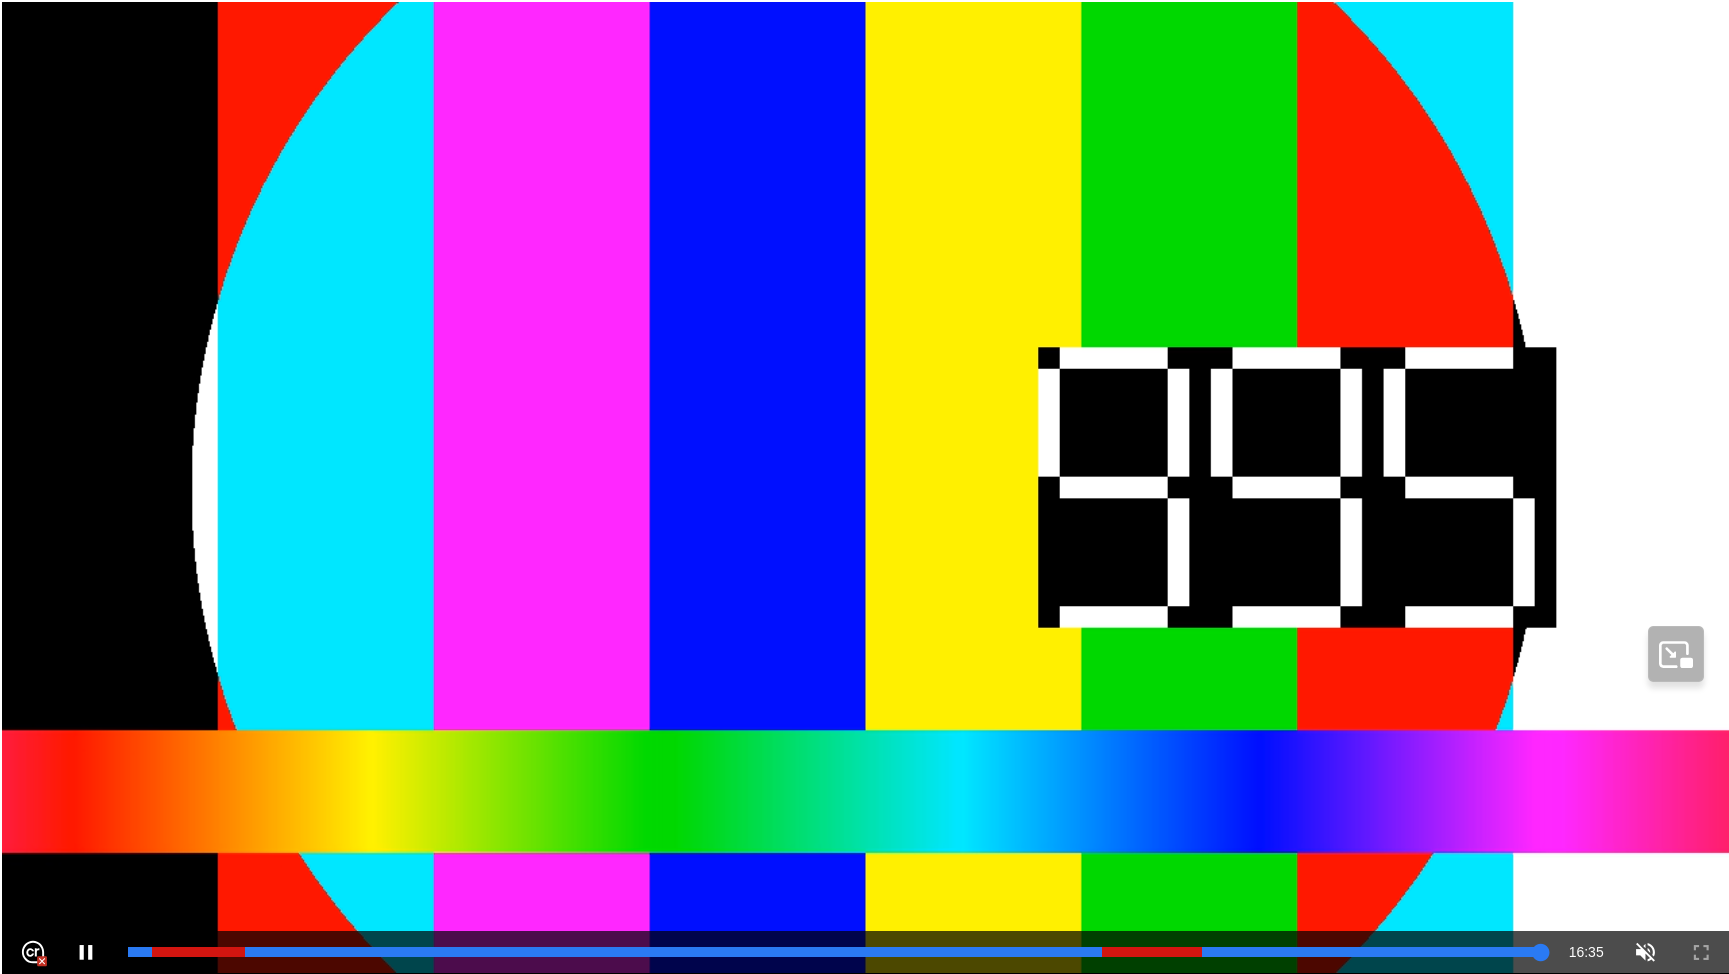
\includegraphics[width=0.95\linewidth, fbox]{videojs-styling.png}
    \caption{Seekbar Video Styling}
    \label{fig:seekbar}
\end{figure}
\begin{figure}
    \centering
    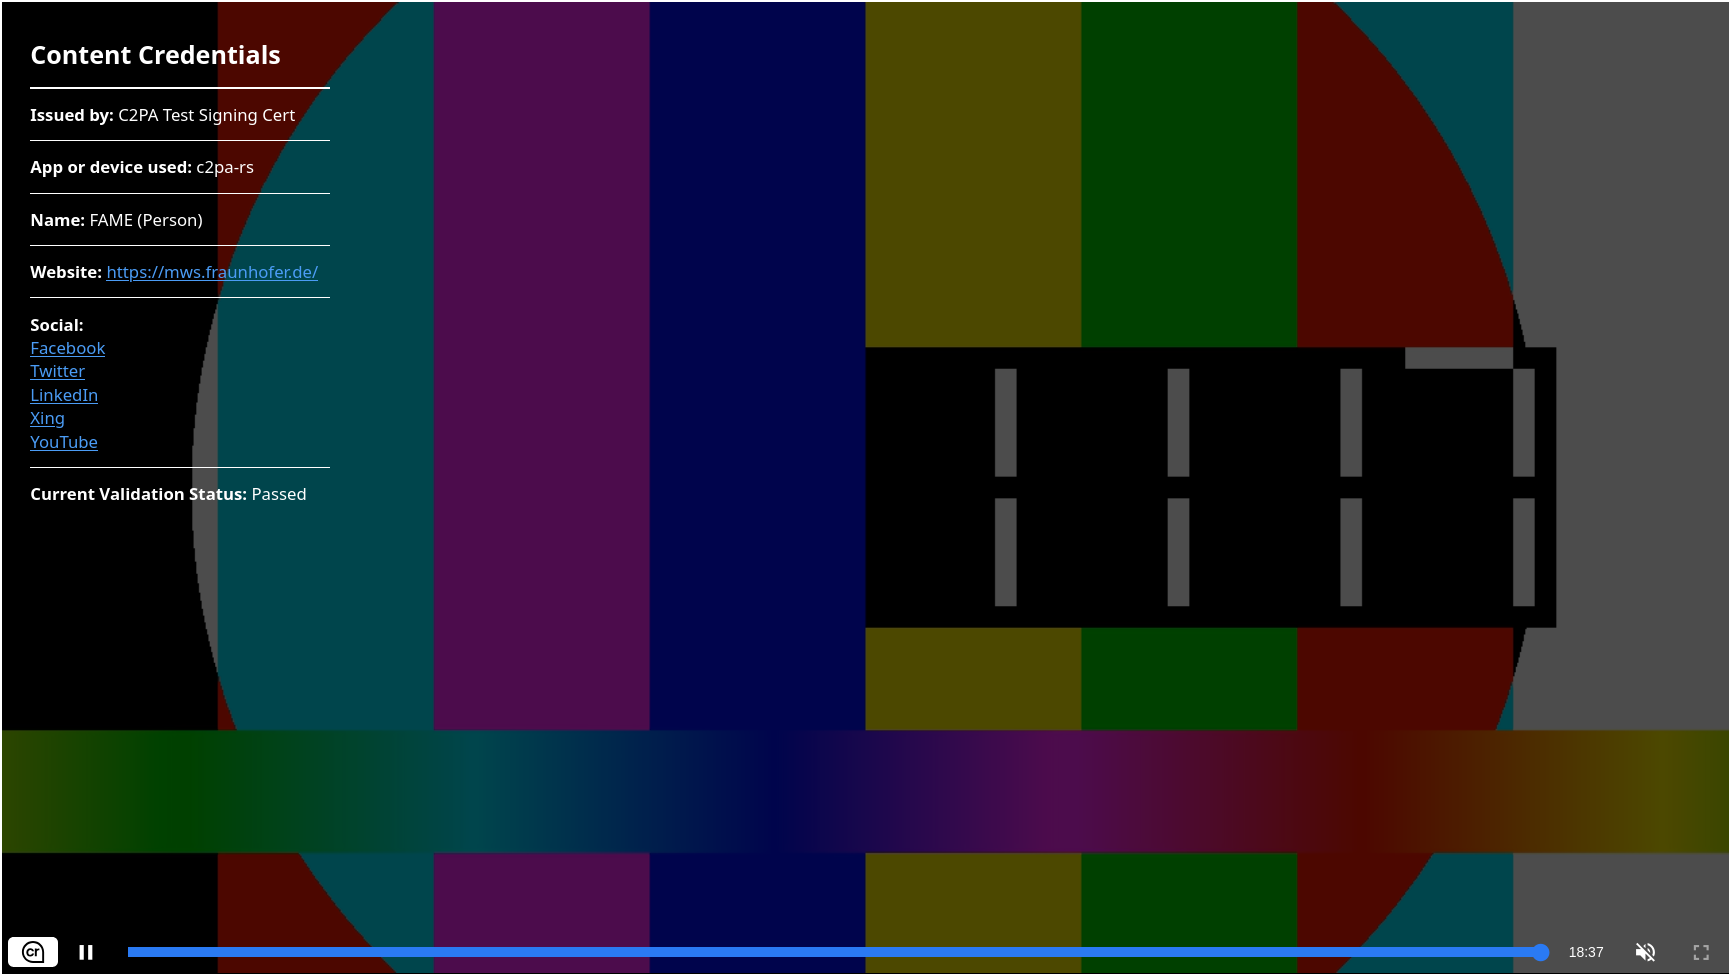
\includegraphics[width=0.95\linewidth, fbox]{overlay-success.png}
    \caption{Video Content Credentials Overlay}
    \label{fig:overlay-success}
\end{figure}
\begin{figure}
    \centering
    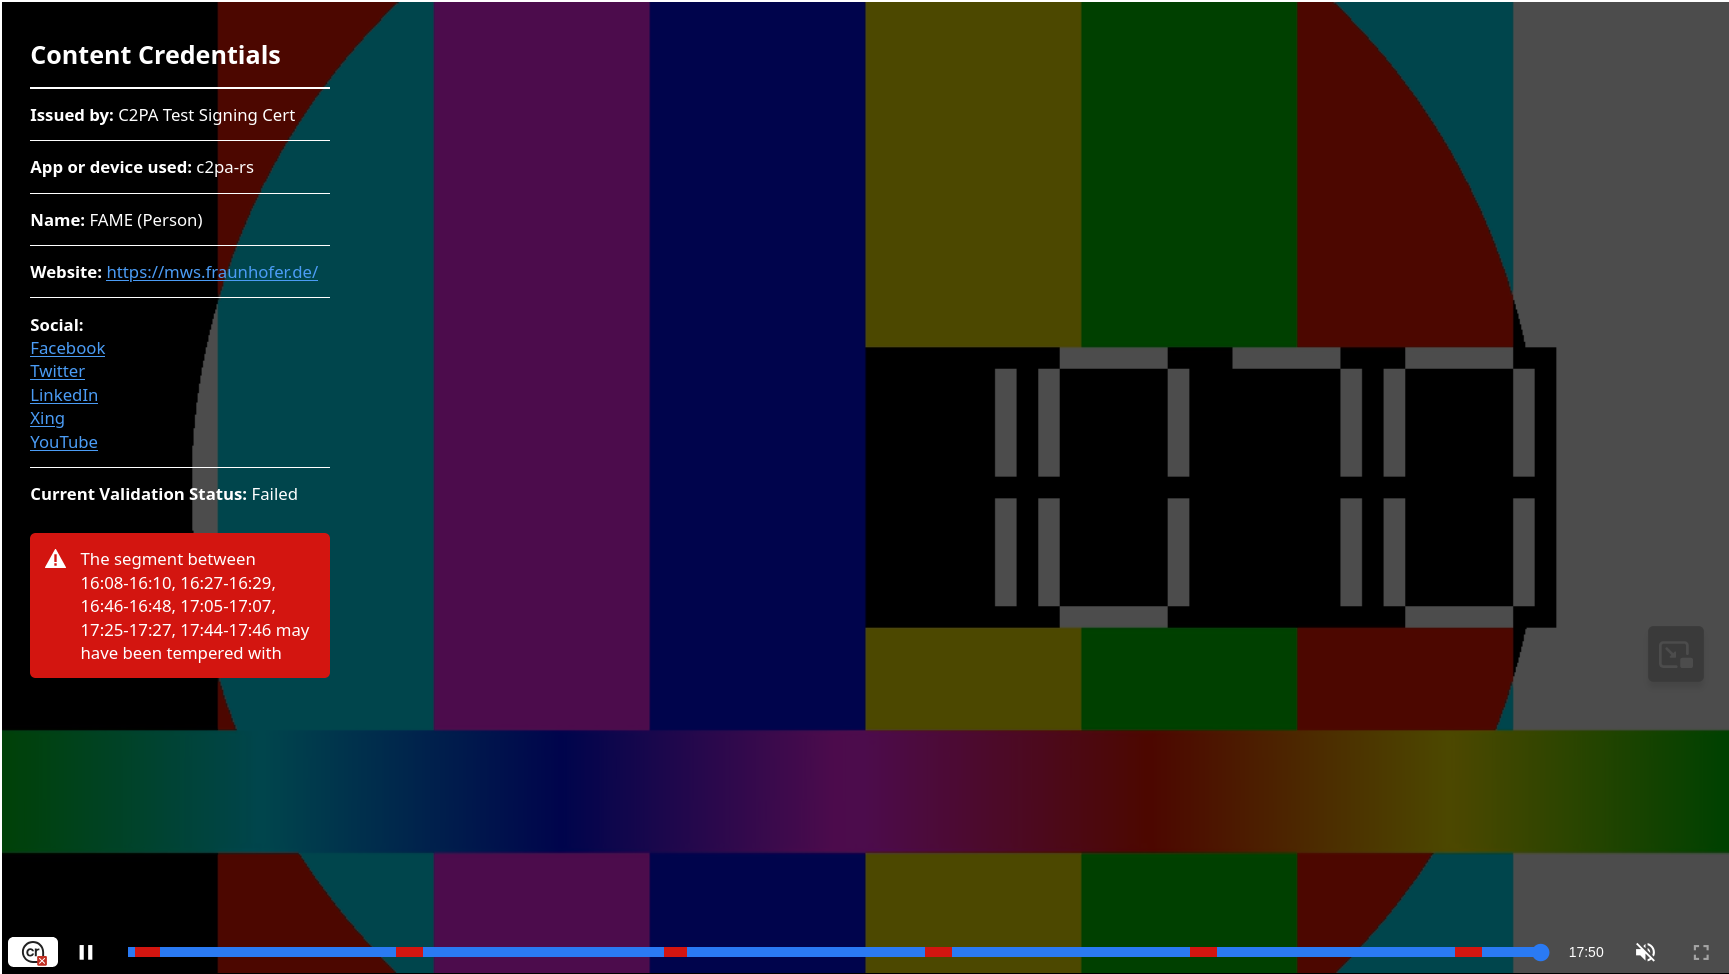
\includegraphics[width=0.95\linewidth, fbox]{overlay-failure.png}
    \caption{Video Content Credentials Overlay With Errors}
    \label{fig:overlay-failure}
\end{figure}

\subsection{Reading the \texttt{c2pa.hash.bmff.v2} Assertion}

Reading the "\texttt{c2pa.hash.bmff.v2}" assertion proved to be a spiteful challenge. Initially, when I was done with the implementation and wanted to test it out, I would always get the result that none of the fragments would correctly validate with trustworthy C2PA manifests.

The culprit ended up being the definition of the \texttt{BmffHash} Rust structure. It uses the popular Rust crate \texttt{serde} (from \textbf{Ser}ialize and \textbf{De}serialize) to define how the structure is converted to and from binary data and in this definition the data field signifying the version is being ignored from the conversion. This resulted that when deserializing this assertion from the previously signed output the version would always be left uninitialized on the structure. This in-turn had the effect that the required version 2 would not be used for all the data hashing, resulting in the erroneous validations.

I fixed this problem by making the existing method \texttt{BmffHash::set\_bmff\_version} public and manually setting the version to \texttt{2} after the assertion had been extracted.

\subsection{CDN Caching\label{sec:caching}}

The Distributor is simple HTTP server built with the \texttt{Rocket}\footnote{Rocket GitHub: \url{https://github.com/rwf2/Rocket}} Rust crate. The media distribution is handled by two endpoints: "\texttt{/ingest/uri...}" and "\texttt{/digest/uri...}". The ingest endpoint is used by the Signer to post the live stream after signing. The digest endpoint is used by the media players on the Consumer to get the published live stream.

To keep the forwarding delay to a minimum the most recent fragments are kept in memory of the Distributor as part of a proxy cache. This cache consists of two components a \texttt{DashMap} and a \texttt{ReplayChannel}. The \texttt{DashMap} is provided by the \texttt{dashmap}\footnote{dashmap GitHub: \url{https://github.com/xacrimon/dashmap}} Rust crate and is essentially a standard Rust \texttt{HashMap} that has been highly optimized for concurrency. The \texttt{ReplayChannel} is taken from the \texttt{replay-channel}\footnote{replay-channel GitHub: \url{https://github.com/freenet/replay-channel}} Rust crate and works just like normal broadcast data channels in Rust with the added caveat that subscribers to that channel will always receive all data starting at the beginning of the channel. With this cache the CDN is able to write fragments to the cache, identified by their URIs, as they arrive. When the Consumer requests a new fragment, the CDN can check if the requested URI is cached. If it is cached I can subscribe to the corresponding channel and send the data as response. When a fragment wasn't cached the CDN will instead read the fragment from local storage.

I make use of the \texttt{FFmpeg} arguments \texttt{-window\_size <num>} and \texttt{-extra\_window\_size <num>} to prevent the cache from caching unnecessarily many fragments and stop it from growing too large. The window size argument denotes the number of fragments kept in the DASH manifest and HLS media playlist. The extra window size option defines the number of fragments in addition to window size that are kept saved on the disk. Since I am using an HTTP output, instead of directly deleting the fragments, FFmpeg will instead send an HTTP DELETE request for the corresponding fragment. The Signer forwards these delete requests to the CDN where the denoted fragment is removed from the cache. Additionally, the CDN should not directly delete the fragment from the cache, instead it should save the data to the attached storage. However, since I configured the Signer and CDN to use the same local directly as storage, I am skipping this part in the CDN to prevent unnecessary redundant IO operations.

\subsection{Producer Inputs\label{sec:producer_inputs}}

The Producer is capable of accepting a variety of input types. The input can be configured using the CLI arguments as shown in \Cref{sec:cli_producer}.

\subsubsection{Remote}

Remote inputs can be anything that is addressable using an IP-compliant address. Examples for this are URLs pointing to server hosted DASH MPDs or HLS Playlists which denote VoDs or live streaming, IP-cameras like the Android app DroidCam \footnote{DroidCam Homepage: \url{https://droidcam.app/}}, which turns your smartphone into a camera or anything else that is supported as input by \texttt{FFmpeg}.

\subsubsection{Local}

Video files are the local input type. They can be either used as a static input to created a limited time stream or they can be used a infinite loop to create a endless live stream.

\subsubsection{Standard Input}

This input option expects raw images on the standard input pipe, which turn these images into a video stream. In this use case \texttt{FFmpeg} expects a definition of the image resolution to properly interpret the received data. This type was needed by a different project where the images were created by the Unity Game Engine\footnote{Unity Homepage: \url{https://unity.com/}} and then used to create a live stream for a remote rendering scenario.

\subsubsection{Device}

On Linux video devices are addressed using a path, for example contents of the \texttt{/dev/} directory, and they can also be used as an input. For example on a laptop with an integrated webcam that webcam is usually the device \texttt{/dev/video0}.

When using this input I had to use the tool \texttt{video4linux2} to extract metadata about the device, like supported formats, resolutions and framerates which are required by \texttt{FFmpeg} to properly parse the input data.

\subsubsection{External Camera\label{sec:ext_cam}}

This method uses the same \textbf{Device} input as detailed in the previous section but since getting this to work required more work, I am giving it its own section.

For this thesis I was provided with a Sony Alpha 7 III, so these steps apply only to this specific camera (every vendor likely has different implementations of getting this working).

Normally, Sony provides the software tool Imaging Edge Webcam \footnote{Imaging Edge Webcam Product Page: \url{https://support.d-imaging.sony.co.jp/app/webcam/en/}}, which turns the camera into a webcam when connected to a PC. Unfortunately, this program is only supported on Windows and macOS operating systems, as described on the download page, and I am using a Linux operating system. However, I was able to find a Reddit thread, which had a comment detailing a workaround to get an alternative working \footnote{Reddit - Sony Imaging Edge Webcam in Ubuntu: \url{https://www.reddit.com/r/Ubuntu/comments/s4zjo7/comment/kwsoxzm/}}.

This approach uses the tool \texttt{gphoto2} \footnote{gPhoto Homepage: \url{http://gphoto.org/}}, an open source application for digital cameras and media players on Unix-like systems. The first step is installing the required tools \texttt{gphoto2}, \texttt{video4linux2 loopback-utils} and \texttt{FFmpeg} by running \texttt{sudo apt install gphoto2 v4l2loopback-utils ffmpeg}, followed by plugging in the camera using an USB cable. If the file system automatically mounts the camera, it is important to unmount it. It is important to then select the option to use the camera as capture device when prompted to on the camera's display, instead of using it to transfer files to the connected device. The next step is creating a new video device using the video feed from the camera. Before the device can be created it is important to be able to determine which device is being created by this process: first ensure no other loopback service is running by stopping the service using the command \texttt{sudo rmmod v4l2loopback}. Next, determine the currently available video devices by remembering the list given by \texttt{ls /dev/video*}. Now start the loopback service using the camera's video feed with the command \texttt{sudo modprobe v4l2loopback exclusive\_caps=1 max\_buffers=2} to create the new video device. The designation of this device can be determined by listing the available video device again (with the same command as before). Whatever device that is now on this list that wasn't there before is the device that was created by this process. Whether this process has worked can be verified by running \texttt{gphoto2 --auto-detect}. If the process was successful, the terminal should now display the camera model name and the port it is connected to. Finally, the last step is actually piping the video feed from the camera to the video device by running the final command \texttt{photo2 --stdout --capture-movie | ffmpeg -i - -vcodec rawvideo -pix\_fmt yuv420p -threads 0 -f v4l2 <video device>}. 

Once this command is running the camera feed is now accessible from the specified video device.

I have automated this process in the helper shell script. I split this process up into two additional shell scripts in the Producer repository: setup and run-capture. The setup encompasses everything after the dependency installation up until the final piping command. It stops the possibly running loopback services, reads the currently running video devices and keeps them in memory, then it starts the loopback service, reads the available devices again, then it filters out all video devices that are new in the second reading. Finally, when multiple new devices have been found, it prompts the use to choose which device to use. Otherwise, it will automatically use the one device found. The determined video device path will be printed to the standard output. The run-capture script expects the video capture device path argument and will simply run the final piping command.

The automation starts by calling the setup script and saving the returned video device to a variable. Then it starts the run-capture script in a separate terminal using \texttt{gnome-terminal -- ./run-capture \$VIDEO\_DEVICE}. Finally, I am waiting five seconds to make sure that the video device is saturated. 

\section{Documentation\label{sec:docu}}

To effortlessly run this testbed during development, I have created four helper shell scripts. Each of these scripts corresponds to one of the four components of this testbed. They are pre-configured with options, which allow running the testbed without needing specific knowledge of the CLI options of all the components. 

However, it is still possible to overwrite some of the default values, specifically only for the Signer and CDN scripts. This can be achieved using environment variables. For example on Linux, if one wants to use port 7000 instead of the default port of the CDN, the script command would like the following: \texttt{PORT=7000 ./scripts/cdn}. When setting multiple overwrites the individual environment variable declarations are separated by a whitespace.

\subsection{Producer}

The \texttt{./scripts/producer} does not use environment variables to overwrite default values. Instead it uses a similar CLI interface to the actual Rust programs. By default, if no arguments given, the producer will use the test image as input. To configure it, the first argument is a subcommand followed by an optional input value. 

All available options are:

\begin{itemize}
    \item Test:
    \begin{itemize}
        \item Command: test
        \item Input: none
        \item Description: use a test image as input (default behavior if no command given)
    \end{itemize}
    \item Webcam:
    \begin{itemize}
        \item Command: webcam
        \item Input: none
        \item Description: use \texttt{/dev/video0} as input device
    \end{itemize}
    \item Device:
    \begin{itemize}
        \item Command: device
        \item Input: capture device path
        \item Description: same webcam command, but with a specific capture device
    \end{itemize}
    \item Local:
    \begin{itemize}
        \item Command: local
        \item Input: path to local video file
        \item Description: use the local video file as input
    \end{itemize}
    \item Remote:
    \begin{itemize}
        \item Command: remote
        \item Input: URL to remote resource
        \item Description: use the remote resource as input
    \end{itemize}
    \item DroidCam:
    \begin{itemize}
        \item Command: droidcam
        \item Input: none
        \item Description: use the default address of the DroidCam Android app as input 
    \end{itemize}
    \item External:
    \begin{itemize}
        \item Command: external
        \item Input: none
        \item Description: use an external cameras as input (this will run the script described in \Cref{sec:ext_cam})
    \end{itemize}
    \item Help:
    \begin{itemize}
        \item Command: help
        \item Input: none
        \item Description: print a help page describing these exact commands 
    \end{itemize}
\end{itemize}

This script must be launched after both the Signer and CDN are running, otherwise the output will point to a non-existing target and FFmpeg will crash.

\subsection{Signer}

The \texttt{./scripts/signer} script will run the \texttt{c2patool} in live signing mode. Configuration options are the address of the CDN ingest URL, which should be the address the CDN is using, the output directory where to save the data to, the path to the C2PA Manifest JSON definition file and the window size for the optimize Merkle Tree signing. This script must be running before starting the Producer.

\begin{table}[H]
    \centering
    \begin{tabular}{|r|l|l|}
    \hline
    \multicolumn{1}{|l|}{\textbf{Variable}} & \textbf{Value} & \textbf{Description}                                                                    \\ \hline
    CDN                                     & URL            & CDN ingest URL                                                                          \\ \hline
    OUTPUT                                  & Path           & Path to save directory                                                                  \\ \hline
    MANIFEST                                & Path           & \begin{tabular}[c]{@{}l@{}}Path to C2PA Manifest JSON\\ definition file\end{tabular}    \\ \hline
    WINDOW                                  & usize          & \begin{tabular}[c]{@{}l@{}}Window size for optimized\\ Merkle Tree signing\end{tabular} \\ \hline
    \end{tabular}
    \caption{Signer Environment Variables}
\end{table}

\subsection{CDN}

The \texttt{./scripts/cdn} starts the CDN server. It can be configured with a different localhost port or the address can be overwritten entirely (in this case the port variable has no effect) and the output directory can be specified. This script must be running before starting the Producer. The order of running the Signer or CDN first does not matter.

\begin{table}[H]
    \centering
    \begin{tabular}{|r|l|l|}
    \hline
    \multicolumn{1}{|l|}{\textbf{Variable}} & \textbf{Value}                                           & \textbf{Description}                                                                        \\ \hline
    PORT                                    & u16                                                      & Localhost Port on which to listen                                                           \\ \hline
    BIND                                    & \begin{tabular}[c]{@{}l@{}}Socket\\ Address\end{tabular} & \begin{tabular}[c]{@{}l@{}}he Socket Address on which\\ the CDN will listen on\end{tabular} \\ \hline
    MEDIA                                   & Path                                                     & \begin{tabular}[c]{@{}l@{}}The path to the output \\ directory\end{tabular}                 \\ \hline
    \end{tabular}
    \caption{CDN Environment Variables}
\end{table}

\subsection{Consumer}

The \texttt{./scripts/consumer} script is the easiest of all the scripts and does not require any configuration. This script will run the SvelteKit website and open it automatically in the default web browser. The will try to use to port \texttt{5173} of localhost and if that is not available, it will automatically increment the port by \texttt{1} until it finds an available port.

This script can be run whenever one wants.
